\chapter{Fizikai modell}\label{chap:physical_system}

Ebben a fejezetben a robot egyetlen motorjának fizikai modellje kerül bevezetésre. A kapott dinamikai leírás
lehetővé teszi az időkéséssel kiegészített stabilitásvizsgálatot. 

\section{Egyenáramú motor dinamikája}

\begin{figure}[h]
\begin{center}
%\phantomsection{}
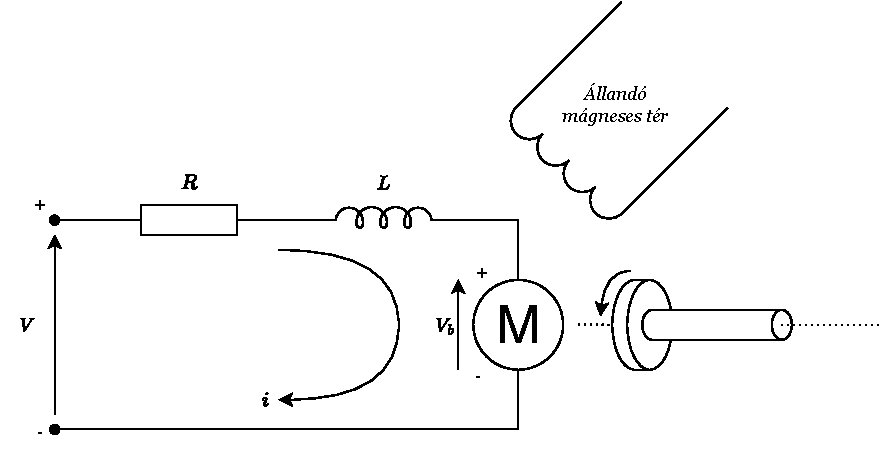
\includegraphics[width=\textwidth]{images/motor_model_electric.pdf}
\caption{Az gyenáramú motor áramköri diagramja}
\label{fig:dc_motor_electric}
\end{center}
\end{figure}

A robot motorjának modelljét a~\ref{fig:dc_motor_electric}-es ábra mutatja. A felhasznált motor feltételezetten állandó gerjesztésű. A kifejtett nyomaték 
a Biot--Savart-törvény szerint arányos a forgórészen átfolyó árammal. A forgórészben
indukált feszültség pedig arányos annak szögsebességével. A Lenz-törvény alapján 
\begin{equation}
\begin{split}
    \tau_\RM m &= K_\RM \tau i, \\
    V_\RM b &= K_\RM e \dot\theta,
\end{split}
\end{equation}
ahol $K_\RM \tau$ a nyomatékállandó, $K_\RM e$ a sebesség-feszültség állandó, $\tau_\RM m$ a kifejtett 
nyomaték, $i$ a rotor árama, $V_\RM b$ az rotorban indukált feszültség és $\dot\theta$ a rotor szögsebessége.
Az energia-megmaradás törvénye alapján a két konstans értéke megegyezik
\begin{align}
    K_\RM m := K_\RM \tau = K_\RM e,
\end{align}
így a következőkben $K_m$ paraméterként jelennek meg. A forgórész áramkörére Kirchhoff I. törvénye alapján felírható
\begin{align}\label{eq:armature_circuit}
    V - Ri - L\DIFF{i}{t} - K_\RM m\dot\theta = 0,
\end{align}
ahol $R$ a forgórész tekercsének ellenállása, $L$ a tekercs induktivitása, 
$K_m$ a motorállandó, $V$ a motor feszültsége, $i$ a motoráram és $\theta$ a szögelfordulás.
\begin{figure}[h]
    \begin{center}
    %\phantomsection{}
    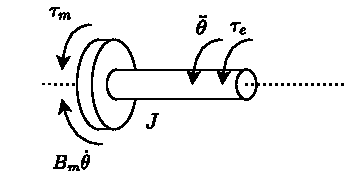
\includegraphics[width=10cm]{images/motor_model_mechanical.pdf}
    \caption{Az egyenáramú motor szabadtest ábrája}
    \label{fig:dc_motor_mechanical}
    \end{center}
\end{figure}
A forgórészt merev testnek tekintve, annak mozgásegyenlete a dinamika alaptétele és a SZTÁ (lásd~\ref{fig:dc_motor_mechanical}. ábra) 
alapján a következő alakban vezethető le:
\begin{align}\label{eq:rotor_dynamics}
    J\ddot\theta = -B_\RM m\dot\theta + \tau_\RM m + \tau_\RM e,
\end{align}
ahol $J$ a forgórész tehetetlensége, $B_\RM m$ a viszkózus csillapítási együttható, 
$K_\RM m$ a motorállandó, $\theta$ a szögelfordulás, $i$ a motoráram, $\tau_\RM m$ a motor által kifejtett nyomaték 
és $\tau_\RM e$ a forgórészre ható külső nyomaték. 
    
A~\eqref{eq:armature_circuit} és~\eqref{eq:rotor_dynamics} egyenletek egyértelműen leírják a 
rendszer időtartománybeli viselkedését.
A további vizsgálathoz kedvezőbb a differenciálegyenleteket állapottér modellként felírni.
Az állapottér modell általánosan
\begin{equation}\label{eq:state_space_generic}
\begin{split}
    \dot{\BF x} &= \BF A \BF x + \BF B \BF u\,,\\
    \BF y &= \BF C \BF x + \BF D \BF u
\end{split}
\end{equation} 
alakban írható fel. Legyen \(\BF x = [\theta~~\dot \theta~~i]^{\mathsf T}\) az állapotvektor, 
\(\BF u = [\tau_\RM e~~V]^{\mathsf T}\) a bemeneti vektor és \(y = \theta\) a kimenet.
A~\eqref{eq:armature_circuit} és a~\eqref{eq:rotor_dynamics} egyenleteket átrendezve 
az állapot-átmeneti mátrix \(\BF A\), a bemeneti mátrix \(\BF B\), a kimeneti mátrix \(\BF C\) és a segédmátrix \(\BF D\) 
\begin{equation}\label{eq:state_space}
    \begin{split}
        \BF A &= 
        \begin{bmatrix}
            0 & 1 & 0 \\
            0 & -\frac{B_\RM m}{J} & \frac{K_\RM m}{J} \\
            0 & -\frac{K_\RM m}{L} & -\frac{R}{L} \\
        \end{bmatrix}\,,\\
        \BF B &=
        \begin{bmatrix}
            0 & 0 \\
            1 & 0 \\
            0 & 1 \\
        \end{bmatrix}\,,\\
        \BF C &=
        \begin{bmatrix}
            1 & 0 & 0 \\
        \end{bmatrix}\,,\\
        \BF D &= \BF 0
    \end{split}
\end{equation}
alakban származtatható.

A frekvenciatartománybeli vizsgálatokhoz szükséges felírni a rendszer 
szög-nyomaték és szög-feszültség átviteli függvényeit. Az állapottér modellt felhasználva
\begin{align}\label{eq:transfer_generic}
    \frac{Y(s)}{U(s)} = \BF C{\left(s \BF I - \BF A\right)}^{-1} \BF B
\end{align}
általános formában, ahol $\BF I$ az identitás mátrix. Behelyettesítve~\eqref{eq:state_space} 
paramétereit~\eqref{eq:transfer_generic} alapján a karakterisztikus polinom felírható
\begin{align}\label{eq:characteristic_polynomial}
    p(s) = s\left(JLs^2 + \left(B_\RM m L + JR\right)s + K_\RM m^2 + B_\RM m R\right)
\end{align}
alakban. Az átviteli függvények pedig ez alapján
\begin{equation}\label{eq:transfer_function}
    \begin{split}
        \frac{\theta(s)}{\tau_\RM e(s)} &= \frac{Ls + R}{p(s)}\,,\\
        \frac{\theta(s)}{V(s)} &= \frac{K_\RM m}{p(s)}.
    \end{split}
\end{equation}

\section{Egyenáramú motor stabilitása}
A motor stabilitása a~\eqref{eq:characteristic_polynomial} egyenletben szereplő karakterisztikus 
polinom segítségével meghatározható.
A karakterisztikus polinom egyik zérusa az origóban helyezkedik el. Ebből következik, hogy a rendszer
egységugrás bemenetre korlátlanul nagy szögelfordulással válaszol. Ez utóbbi a Ez a jelen alkalmazásban nem elfogadható. 
Ha a szabályozókör visszacsatoló ága megszakad, a motor a megengedhető mozgástartományon kívülre fordulhat.
A biztonságos működéshez szükséges például egy végálláskacsolót beépíteni, mely segítségével a motor 
mozgástartománya mechanikailag is az előírt tartományon belülre korlátozható.
